\documentclass[10pt,twocolumn]{article}
\usepackage[margin=0.75in]{geometry}
\usepackage{amsmath,amssymb,amsthm,bm,mathtools}
\makeatletter\let\tabinput\@@input\makeatother
\usepackage{graphicx,booktabs,multirow,xcolor}
\usepackage[hidelinks]{hyperref}
\usepackage{braket}
\usepackage{tikz}
\usetikzlibrary{positioning,arrows.meta,calc,decorations.pathreplacing}
\usepackage{natbib}
\usepackage{caption}
\captionsetup{font=small}
\newtheorem{proposition}{Proposition}
\newtheorem{lemma}{Lemma}
\theoremstyle{remark}
\newtheorem*{remark}{Remark}
\newcommand{\E}{\mathbb{E}}
\newcommand{\SWAP}{\mathrm{SWAP}}

\title{Exchange-Only Quantum Discrete Diffusion for Language Modeling}
\author{Yuichiro Minato\\ \small blueqat Inc.}
\date{}

\begin{document}
\maketitle

\begin{abstract}
We build a discrete diffusion language model whose only quantum operation is the Heisenberg exchange
interaction, the native gate of semiconductor spin qubits. Each token is a single spin excitation among
$V$ qubits. The uniform D3PM corruption process is realised exactly as a random spin-shuffling
(SWAP) channel, and the denoiser is an exchange circuit whose pulse areas are set by the noisy context.
Measuring the circuit samples the clean token by the Born rule, so ancestral sampling needs a single shot
per token and step. We show that exchange acts on the token register through the dynamical Lie algebra
$\mathfrak u(V-1)$: the $W$ state is dark, and every output obeys an amplitude sum rule. Nevertheless,
every categorical distribution remains reachable, and nearest-neighbour hardware needs depth of at
least $V-1$. Using an exact simulator for 32-qubit registers, we train character-level models on
$2\times10^6$ characters and compare them with classical denoisers that use identical features. The
exchange read-out reaches $3.38\pm0.01$ (linear controller) and $3.18\pm0.01$ (MLP controller)
bits/char, about $0.25$~bits/char behind softmax read-outs ($3.13$ and $2.92$). In return, the one-hot
register makes relaxation and single readout flips detectable. Under exactly simulated noise, a 1\%
readout error costs $0.012$~bits/char with a Hamming-weight check versus $0.29$ for a binary code. With
the same check, relaxation affecting 80\% of shots costs only $0.03$~bits/char. The model is classically
simulable by construction, so we claim no quantum advantage; all code and results are released.
\end{abstract}

\section{Introduction}
Diffusion models \citep{sohl2015deep,ho2020denoising} have been extended to discrete data by
replacing Gaussian noise with Markov transition matrices on a finite vocabulary
\citep{austin2021structured,hoogeboom2021argmax}, and discrete diffusion is now a competitive
non-autoregressive approach to language modeling \citep{lou2024discrete,sahoo2024simple}.
In parallel, several quantum versions of diffusion models have been proposed, in which either the data
are quantum states or the denoiser is a parameterised quantum circuit
\citep{zhang2024generative,parigi2023quantum,cacioppo2023quantum,kolle2024quantum}.
These proposals generally assume a universal gate set with arbitrary single-qubit rotations.

This paper asks a hardware-driven question: \emph{how far can a discrete diffusion language model go
if the only operation available is the Heisenberg exchange interaction?} Exchange is the native
two-qubit interaction of semiconductor spin qubits \citep{loss1998quantum,burkard2023semiconductor}.
``Exchange-only'' architectures avoid fast single-spin control altogether and recover universality by
encoding logical qubits in several spins \citep{divincenzo2000universal,weinstein2023universal}.
Here we take a different route. We do not try to recover universality. Instead, we pick a data
encoding in which exchange alone is already the natural set of operations for a categorical
distribution over tokens.

\paragraph{Idea.} A token from a vocabulary of size $V$ is stored as a single spin excitation among
$V$ qubits (one-hot or unary encoding). Exchange conserves the number of excitations, so every exchange
circuit acts inside the $V$-dimensional single-excitation sector. There it implements a unitary
``mixing'' of tokens. A random exchange (SWAP) channel corrupts tokens exactly as the uniform D3PM forward
process does. A trained, context-dependent exchange circuit followed by a computational-basis
measurement samples the denoised token by the Born rule.

\paragraph{Contributions.}
(i) We formulate an exchange-only quantum discrete diffusion model (QXDM) with a one-hot token
register, an exchange-channel forward process, a Born-rule denoiser and measurement-based ancestral
sampling that needs \emph{one shot per token per step}.
(ii) We characterise its expressivity. The dynamical Lie algebra on the token register is
$\mathfrak{u}(V\!-\!1)$, and the $W$ state is a dark state. This imposes an exact amplitude sum rule.
Despite this, every categorical distribution remains reachable as a single Born-rule output, and
nearest-neighbour hardware has a light-cone depth requirement.
(iii) We give an exact and efficient simulator (single-excitation dynamics are classically simulable)
and use it to train character-level models on $2\times 10^6$ characters. We compare them with
classical denoisers that share the same features.
(iv) We study realistic exchange-only noise. Charge noise, dephasing, relaxation and readout errors
are all simulated exactly. The one-hot encoding turns relaxation and single readout flips into
\emph{detectable} errors through a Hamming-weight check.

We stress at the outset that the model class studied here is classically simulable by construction,
so we make no claim of quantum advantage. Our goal is a hardware-native, verifiable baseline. It shows
what an exchange-only device can and cannot express when it is used as the stochastic core of a
generative language model.

\section{Background}
\paragraph{Uniform discrete diffusion.}
Let $x_0\in\{1,\dots,V\}^L$ be a sequence. The uniform forward process corrupts each token
independently,
$q(x_t\,|\,x_{t-1}) = \mathrm{Cat}\big(\alpha_t e_{x_{t-1}} + (1-\alpha_t)\mathbf{1}/V\big)$,
so that $q(x_t|x_0)=\mathrm{Cat}(\bar\alpha_t e_{x_0}+(1-\bar\alpha_t)\mathbf{1}/V)$ with
$\bar\alpha_t=\prod_{s\le t}\alpha_s$ \citep{austin2021structured,hoogeboom2021argmax}. We use $T=32$
steps, a cosine schedule and $\bar\alpha_T=0$, so $x_T$ is exactly uniform. A denoiser
$p_\theta(x_0|x_t)$ defines the reverse kernel
\begin{equation}
p_\theta(x_{t-1}|x_t)=\sum_{\hat x_0} p_\theta(\hat x_0|x_t)\, q(x_{t-1}|x_t,\hat x_0),
\label{eq:rev}
\end{equation}
factorised over positions. The negative evidence lower bound (NELBO) is
$\sum_{t\ge2}\E\,\mathrm{KL}\big(q(x_{t-1}|x_t,x_0)\,\|\,p_\theta(x_{t-1}|x_t)\big)
-\E\log p_\theta(x_0|x_1)$. The prior term vanishes because $\bar\alpha_T=0$. Eq.~\eqref{eq:rev} is
exactly the law of ``draw $\hat x_0\sim p_\theta(\cdot|x_t)$, then draw $x_{t-1}$ from the analytic
posterior''. This is what makes a sampling-only (Born-rule) denoiser natural.

\paragraph{Exchange interaction.}
For spins $a,b$ the isotropic exchange Hamiltonian is
$H_{ab}=\tfrac{J}{4}\,\bm\sigma_a\!\cdot\!\bm\sigma_b$, which equals $\tfrac{J}{2}\SWAP_{ab}$ up
to a constant. A pulse therefore implements
\begin{equation}
E_{ab}(\theta)=e^{-i\theta\,\SWAP_{ab}}=\cos\theta\,\mathbb 1-i\sin\theta\,\SWAP_{ab},
\end{equation}
with $\theta=\int J\,dt/2$. Exchange commutes with every global spin rotation, so it conserves both the
total spin $S^2$ and the magnetisation $S_z$ \citep{divincenzo2000universal,marvian2022restrictions}.

\section{Exchange-only quantum discrete diffusion}
\begin{figure}[t]
\centering
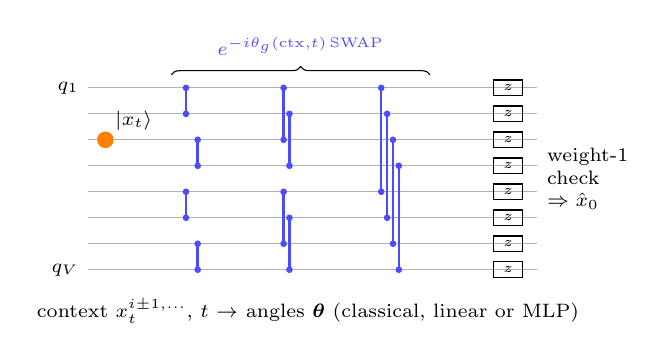
\begin{tikzpicture}[x=0.62cm,y=0.33cm,font=\scriptsize]
  \foreach \q in {0,...,7} {\draw[gray!60] (0,-\q) -- (9.2,-\q);}
  \node[left] at (0,0) {$q_1$}; \node[left] at (0,-7) {$q_V$};
  \fill[orange] (0.35,-2) circle (3pt); \node[above right] at (0.35,-2) {$\ket{x_t}$};
  % butterfly layers
  \foreach \l/\s in {1/1,2/2,3/4} {
    \foreach \a in {0,...,7} {
      \pgfmathtruncatemacro{\bit}{mod(floor(\a/\s),2)}
      \ifnum\bit=0
        \pgfmathsetmacro{\xx}{\l*2.0+0.12*mod(\a,4)}
        \draw[blue!70,line width=0.9pt] (\xx,-\a) -- (\xx,-\a-\s);
        \fill[blue!70] (\xx,-\a) circle (1.2pt); \fill[blue!70] (\xx,-\a-\s) circle (1.2pt);
      \fi
    }
  }
  \node[blue!70] at (4.35,1.6) {$e^{-i\theta_g(\mathrm{ctx},t)\,\mathrm{SWAP}}$};
  \draw[decorate,decoration={brace,amplitude=3pt}] (1.7,0.5) -- (7.0,0.5);
  \foreach \q in {0,...,7} {\draw (8.3,-\q-0.3) rectangle (8.9,-\q+0.3); \node at (8.6,-\q) {\tiny$z$};}
  \node[right,align=left] at (9.2,-3.5) {weight-1\\check\\$\Rightarrow\hat x_0$};
  \node[align=center] at (4.5,-8.6) {context $x_t^{i\pm1,\dots}$, $t$ $\to$ angles $\bm\theta$ (classical, linear or MLP)};
\end{tikzpicture}
\caption{Exchange-only denoiser for one token. The noisy token $x_t^i$ is loaded as a single excitation
on $V$ qubits. Layers of exchange pulses with context-dependent angles (here a butterfly network, i.e.\
$\log_2 V$ layers per block) act inside the single-excitation sector. A $z$-basis measurement with a
Hamming-weight check returns $\hat x_0\sim|\braket{\hat x_0|U|x_t^i}|^2$, which is fed to the analytic
posterior $q(x_{t-1}|x_t,\hat x_0)$.}
\label{fig:schematic}
\end{figure}

\subsection{Token register}
Each sequence position owns a register of $V$ qubits. The token $k$ is stored as
$\ket{e_k}=\ket{0\cdots010\cdots0}$ (excitation on qubit $k$). Let $\mathcal H_1=\mathrm{span}\{\ket{e_k}\}$.

\begin{lemma}[Exchange on the token register]\label{lem:block}
$E_{ab}(\theta)$ leaves $\mathcal H_1$ invariant. On $\mathcal H_1$,
$E_{ab}(\theta)=e^{-i\theta}\exp(i\theta L_{ab})$, with the edge Laplacian
$L_{ab}=(e_a-e_b)(e_a-e_b)^{\!\top}$. Explicitly, up to the global phase the gate acts as
$\begin{psmallmatrix}u&v\\v&u\end{psmallmatrix}$ on $(e_a,e_b)$, where $u=e^{i\theta}\cos\theta$ and
$v=-ie^{i\theta}\sin\theta$, and as the identity on all other $e_k$.
\end{lemma}
\begin{proof}
$\SWAP_{ab}$ permutes $e_a\leftrightarrow e_b$ and fixes the other $e_k$, so on $\mathcal H_1$ we have
$\SWAP_{ab}=\mathbb 1-L_{ab}$. Since $L_{ab}^2=2L_{ab}$,
$e^{i\theta L_{ab}}=\mathbb 1+\tfrac{e^{2i\theta}-1}{2}L_{ab}$, which gives the stated entries.
\end{proof}
Thus a circuit of $G$ exchange pulses is simulated exactly in $O(G)$ time per basis input. Every gate
updates two amplitudes: $\psi_a\!\leftarrow\!\psi_a-\Delta$ and $\psi_b\!\leftarrow\!\psi_b+\Delta$, with
$\Delta=(\sin^2\theta-i\sin\theta\cos\theta)(\psi_a-\psi_b)$. We checked Lemma~\ref{lem:block} against a
full $2^n$-dimensional state-vector simulation with the Heisenberg Hamiltonian
(Table~\ref{tab:verify}).

\subsection{Forward process as an exchange channel}
\begin{proposition}\label{prop:forward}
Let $\Phi_t(\rho)=(1-\beta_t)\rho+\beta_t\,\E_{\pi\sim S_V}[P_\pi\rho P_\pi^\dagger]$, where $P_\pi$
permutes qubits according to a uniformly random permutation. With $\beta_t=1-\alpha_t$, the induced
transition on one-hot states is the uniform D3PM kernel $q(x_t|x_{t-1})$.
\end{proposition}
\begin{proof}
Every permutation is a product of transpositions, i.e.\ full-SWAP exchange pulses $E_{ab}(\pi/2)$ up to
phase. $P_\pi\ket{e_k}=\ket{e_{\pi(k)}}$, and $\pi(k)$ is uniform over $\{1..V\}$ for a uniform $\pi$.
\end{proof}
The forward process is therefore physically an exchange (``spin-shuffling'') channel. Training never
has to run it on hardware, because $q(x_t|x_0)$ has a closed form.

\subsection{Exchange-circuit denoiser}
For position $i$ we load $\ket{e_{x_t^i}}$, apply $U_{\bm\theta}=\prod_g E_{a_gb_g}(\theta_g)$ and
measure. Hence
\begin{equation}
p_{\bm\theta}(\hat x_0=k\,|\,x_t,t)=\big|\braket{e_k|U_{\bm\theta(x_t,t)}|e_{x_t^i}}\big|^2 .
\end{equation}
The pulse angles are set by a classical controller from sparse features of the \emph{noisy} context:
the tokens at offsets $-4..4$, five neighbour pairs, the time step $t$, and the joint feature
$(t,x_t^i)$. In the \emph{linear} controller, $\theta_g=J_g(t)\sum_{f\in\mathrm{active}}W_{f,g}$, i.e.\
a sum of learned per-feature pulse areas. The \emph{exchange envelope} $J_g(t)$ scales all pulses at
noise level $t$. When $J\to0$ we get $U\to\mathbb 1$, which implements ``copy $x_t$'' at low noise.
The nonlinear (Born-rule) map from angles to probabilities is performed entirely by the exchange circuit.
As an ablation we also use \emph{data re-uploading} \citep{perez2020data}: each active feature drives
its own exchange block and the blocks are applied in sequence. To isolate the read-out, we further pair
the circuit with a two-layer \emph{MLP controller}. This is the same network as our classical MLP
baseline, but its output is $G$ angles instead of $V$ logits.

We use two connectivities. A \emph{butterfly} network pairs $k\leftrightarrow k\oplus2^s$ in layer
$s=0,\dots,\log_2V-1$; the default is 3 blocks, i.e.\ 15 layers and 240 gates for $V=32$. A
\emph{1D chain} uses nearest-neighbour brick-wall layers, which suits linear quantum-dot arrays.

\subsection{Sampling and training}
\paragraph{Measurement-based ancestral sampling.} At step $t$ every position runs its circuit once and
is measured. The classical posterior $q(x_{t-1}|x_t^i,\hat x_0^i)$ is then sampled, and the next round
re-prepares $\ket{e_{x^i_{t-1}}}$. Because Eq.~\eqref{eq:rev} is a mixture over $\hat x_0$, a single
shot per token per step samples the model exactly. No amplitude or probability estimation is required.
Generating $L$ tokens costs $LT$ circuit executions of depth $D$ on $V$ qubits, and positions are
independent within a step.
\paragraph{Training.} We minimise the D3PM hybrid objective
$T\,\mathcal L_{t-1}+\lambda\,\mathrm{CE}(x_0)$ with a single random $t$ per sequence and $\lambda=0.01$
\citep{austin2021structured}. In simulation we differentiate exactly. On hardware, the generator
$\SWAP$ has eigenvalues $\pm1$, so the two-term parameter-shift rule
$\partial_\theta f=f(\theta+\tfrac\pi4)-f(\theta-\tfrac\pi4)$ applies to every exchange angle
\citep{mitarai2018quantum,schuld2019evaluating}. We verified it numerically (Table~\ref{tab:verify}).

\section{Expressivity of exchange on the token register}
\begin{proposition}[Dark state and sum rule]\label{prop:dark}
For any exchange circuit, $U\ket W=\ket W$ (up to the removed global phase), where
$\ket W=V^{-1/2}\sum_k\ket{e_k}$. Consequently $\sum_k\braket{e_k|U|e_x}=1$ for every input $x$.
\end{proposition}
\begin{proof}
$L_{ab}\mathbf 1=0$ for every edge, so each factor $e^{i\theta L_{ab}}$ fixes $\ket W$. Since $U$ is
unitary, $\bra WU=\bra W$, and
$\sum_k\braket{e_k|U|e_x}=\sqrt V\braket{W|U|e_x}=\sqrt V\braket{W|e_x}=1$.
\end{proof}
Physically, $\ket W$ lies in the maximal-spin multiplet ($S=V/2$). The remaining $V\!-\!1$ states of
$\mathcal H_1$ have $S=V/2-1$, and SU(2)-invariant exchange cannot couple the two sectors.
\begin{proposition}[Dynamical Lie algebra]\label{prop:dla}
For a connected interaction graph, the Lie algebra generated by $\{iL_{ab}\}$ on $\mathcal H_1$ is
$\mathfrak u(V\!-\!1)$, acting on $\ket W^\perp$ and trivially on $\ket W$.
\end{proposition}
We verified Proposition~\ref{prop:dla} numerically by computing the Lie closure for chains and butterflies
with $V\in\{4,6,8\}$ (Table~\ref{tab:verify}). In every case the dimension equals $(V-1)^2$, not $V^2$.
\begin{proposition}[Every distribution is reachable]\label{prop:reach}
For any input $x$ and any distribution $p$ on $\{1..V\}$, there is a $U$ in the group generated by
exchange with $|\braket{e_k|U|e_x}|^2=p_k$ for all $k$.
\end{proposition}
\begin{proof}
By Prop.~\ref{prop:dla}, $U$ acts as an arbitrary unitary on $\ket W^\perp$. Hence the reachable outputs
are exactly the unit vectors $\psi$ with $\braket{W|\psi}=\braket{W|e_x}=V^{-1/2}$, i.e.\
$\|\psi\|=1$ and $\sum_k\psi_k=1$. Write $\psi_k=\sqrt{p_k}e^{i\varphi_k}$. Phases with
$\sum_k\sqrt{p_k}e^{i\varphi_k}=1$ exist if and only if segments of lengths $\{\sqrt{p_k}\}\cup\{1\}$
close a polygon. This holds because $\sum_k\sqrt{p_k}\ge\sum_kp_k=1$ and
$\sqrt{p_j}\le1\le 1+\sum_{k\ne j}\sqrt{p_k}$.
\end{proof}
The sum rule therefore does not restrict the set of output distributions. It does restrict
\emph{how} they are parameterised: the amplitudes are coupled through a shared phase constraint, unlike
independent softmax logits. Reachability also needs enough depth. On a nearest-neighbour chain, an
excitation travels at most one site per layer, so with $D<V-1$ layers some outputs have zero
amplitude. Table~\ref{tab:reach} confirms this. Random Dirichlet targets are fitted to a median KL below
$10^{-5}$~nats by a single butterfly block (5 layers) and by a 32-layer chain, but a 16-layer chain
leaves more than 10~nats.
Conversely, the low dimension of the dynamical Lie algebra ($(V-1)^2$, polynomial in $V$) rules out
the exponential concentration associated with barren plateaus \citep{mcclean2018barren,ragone2024lie}.

\section{Noise and error detection}
\label{sec:noise-theory}
Noise in exchange-only spin qubits mainly comes from four sources \citep{burkard2023semiconductor}:
\textbf{(a)} quasi-static charge noise on $J$, i.e.\ $\theta\to\theta(1+\epsilon)$;
\textbf{(b)} dephasing from fluctuating local fields, a random $Z$ phase per qubit and layer;
\textbf{(c)} energy relaxation $\ket1\to\ket0$ with qubit-dependent rate $\gamma_k$ per layer; and
\textbf{(d)} readout bit flips with probability $q$. Channels (a) and (b) preserve $\mathcal H_1$. Channel
(c) maps $\mathcal H_1$ to the vacuum, and (d) acts on classical outcomes. All of them can therefore be
simulated \emph{exactly} for $V=32$ qubits: we use Monte-Carlo averaging over (a, b), the no-jump
trajectory for (c), and closed forms for (d).

\paragraph{Hamming-weight check.} Any valid outcome has Hamming weight 1, so checking the weight is a free
symmetry verification \citep{bonet2018low,mcardle2019error}. A relaxation event yields weight 0 and is
always detected. Post-selection then returns the normalised no-jump state
$\propto\mathrm{diag}(\sqrt{1-\gamma_k})^{D}\,U\ket{e_x}$. In particular, \emph{uniform} relaxation
($\gamma_k\equiv\gamma$) costs only a reduced acceptance rate $(1-\gamma)^D$ and leaves the
model distribution unchanged. For readout flips, a single flip gives weight 0 or 2 and is detected. An
undetected error needs two flips, which happens with probability
$(V\!-\!1)q^2(1-q)^{V-2}=O(Vq^2)$. Compare a dense binary code on $\log_2V$ qubits: there every outcome
is valid, and errors occur undetected with probability $1-(1-q)^{\log_2V}\approx q\log_2V$.

\section{Experiments}
\subsection{Setup}
\paragraph{Data.} We use the English \texttt{fortunes} collection, i.e.\ the data files of the Debian
\texttt{fortunes}/\texttt{fortunes-min} packages, excluding \texttt{ascii-art} and attribution lines.
It is lower-cased and mapped to $V=32$ symbols (\texttt{a--z}, space, \texttt{.\,,\,'\,?\,!}). Entries are
shuffled and split 90/5/5, giving $2.01\times10^6$ training, $1.19\times10^5$ validation and
$1.09\times10^5$ test characters. The unigram entropy is $4.26$~bits.
\paragraph{Models.} All local denoisers share the featuriser of Sec.~3.3 ($F=6{,}831$ sparse
features, 17 active per position). They differ only in the read-out. \emph{Log-linear softmax}: summed
feature logits with a per-$t$ logit scale (the classical analogue of $J(t)$). \emph{MLP softmax}: summed
240-dimensional feature embeddings, two GELU layers, softmax. \emph{Exchange (linear ctrl.)}: summed
pulse areas for $G=240$ exchange gates (butterfly, 3 blocks) with envelope $J(t)$. \emph{Exchange (MLP
ctrl.)}: the MLP above with a 240-angle output feeding the same circuit.
\paragraph{Training and evaluation.} Each run uses Adam \citep{kingma2015adam}, learning rate
$2\times10^{-3}$ (200-step warm-up, cosine decay), $10^4$ steps, and 64 windows of 64 characters per
step. Training is on CPU: about 25~minutes per exchange model on one core, using our real-arithmetic
simulator. We report the test NELBO in bits/char, summing $\mathcal L_{t-1}$ over \emph{all} $T=32$ steps
(no Monte-Carlo over $t$) on 256 test windows. For sample quality we draw 256 unconditional samples of
length 64 by measurement-based ancestral sampling. We score them by (a) their bits/char under an
interpolated Kneser--Ney 5-gram fitted to the training split \citep{chen1999empirical} and (b) the
fraction of interior words of length $\ge2$ that occur in the training vocabulary.

\subsection{Verification of the simulator and theory}
\begin{table}[t]
\centering\small
\caption{Numerical checks. Top: exact agreement of the single-excitation simulator with a full
$2^6$-dimensional Heisenberg simulation of a 4-layer chain, together with the identities used in
Secs.~3--4 (for $V=32$). Bottom: dimension of the dynamical Lie algebra generated by $\{iL_{ab}\}$.}
\label{tab:verify}
\begin{tabular}{lr}
\toprule
max.\ amplitude error vs.\ full $2^6$ state vector & $3.5\times10^{-16}$\\
max.\ leakage out of $\mathcal H_1$ & $0$\\
$\|[U,S^2]\|_{\max}$ & $1.1\times10^{-15}$\\
$\|U\ket W-\ket W\|_{\max}$ (Prop.~\ref{prop:dark}) & $0$\\
sum rule $|\sum_k\braket{e_k|U|e_x}-1|$ & $5.0\times10^{-16}$\\
parameter shift ($\pm\pi/4$) vs.\ autograd & $7.1\times10^{-17}$\\
\bottomrule
\end{tabular}\\[4pt]
\begin{tabular}{lcccc}
\toprule
graph & $V$ & $\dim\mathfrak g$ & $(V-1)^2$ & $V^2$\\
\midrule
\tabinput tables/lie.tex 
\bottomrule
\end{tabular}
\end{table}
\begin{table}[t]
\centering\small
\caption{Column reachability (Prop.~\ref{prop:reach}): KL divergence (nats) after fitting a single
circuit column to 5 random Dirichlet($\alpha$) targets on $V=32$ outcomes. The 16-layer chain is below
the light-cone depth $V-1$.}
\label{tab:reach}
\begin{tabular}{lccc}
\toprule
circuit & $\alpha$ & median KL & max KL\\
\midrule
\tabinput tables/reach.tex 
\bottomrule
\end{tabular}
\end{table}
Table~\ref{tab:verify} confirms Lemma~\ref{lem:block} against a full state-vector simulation with the
Heisenberg Hamiltonian. Leakage is exactly zero and total spin is conserved. The dynamical Lie algebra
has dimension $(V-1)^2$ in every case (Prop.~\ref{prop:dla}). The dark-state and sum-rule identities hold
to machine precision, and the $\pi/4$ parameter-shift rule reproduces automatic differentiation.
Table~\ref{tab:reach} supports Prop.~\ref{prop:reach} and shows the light-cone failure of shallow
nearest-neighbour circuits.

\subsection{Language modeling}
\begin{table*}[t]
\centering\small
\caption{Test NELBO (bits/char; mean $\pm$ s.d.\ over seeds) and sample quality (seed 0, temperature 1).
\emph{Gen.\ bits} is the bits/char of generated text under a Kneser--Ney 5-gram (lower is more
plausible), and \emph{words} is the percentage of generated words found in the training vocabulary. For
reference, the Kneser--Ney 5-gram itself reaches 2.11 bits/char on the test split and the unigram
entropy is 4.26 bits.}
\label{tab:main}
\begin{tabular}{lccccc}
\toprule
denoiser (same features) & params & seeds & test NELBO $\downarrow$ & gen.\ bits $\downarrow$ & words (\%) $\uparrow$\\
\midrule
\tabinput tables/main.tex 
\bottomrule
\end{tabular}
\end{table*}
Table~\ref{tab:main} gives the main result. Seed-to-seed variation is below $0.01$~bits/char. The
exchange denoiser with a linear controller reaches $3.375$~bits/char. A log-linear softmax on the same
features reaches $3.129$, with $7\times$ fewer parameters. Giving both the same nonlinear controller
narrows the absolute numbers but not the gap: $3.177$ for the exchange read-out vs.\ $2.919$ for softmax.
Sample-quality metrics give the same ranking. The MLP softmax produces the most word-like text, while
both exchange models and the log-linear model produce text with about a third valid words and 5-gram
bits/char between 4.6 and 5.0. For comparison, i.i.d.\ unigram text scores $6.41$ and real text $2.22$.
No model collapses: the unigram entropy of every sample set lies between $4.19$ and $4.24$~bits
(data: $4.27$).

\begin{figure}[t]
\centering
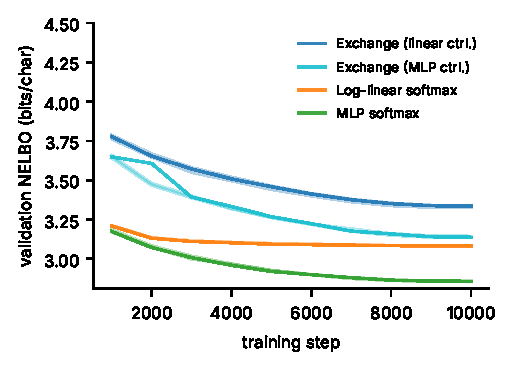
\includegraphics[width=\columnwidth]{figs/curves.pdf}
\caption{Validation NELBO during training (all seeds).}
\label{fig:curves}
\end{figure}
\begin{figure}[t]
\centering
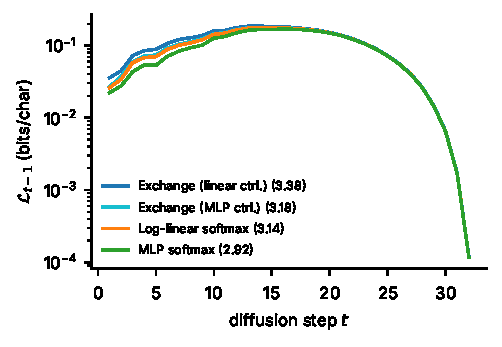
\includegraphics[width=\columnwidth]{figs/per_t.pdf}
\caption{Per-step contribution $\mathcal L_{t-1}$ to the test NELBO (seed 0; totals in the legend). The
exchange read-out loses at every noise level, with the largest relative gap at small $t$, where the
denoiser must copy $x_t$ with high confidence.}
\label{fig:per_t}
\end{figure}

\begin{figure}[t]
\centering\scriptsize
\resizebox{\columnwidth}{!}{%
\begin{tabular}{@{}r@{\;}l@{}}
$t$ & exchange denoiser (linear ctrl.), one sample\\
\midrule
32 & \texttt{flmi!jlfpaqbmhn,gzsu?fsul,k,'osexxjrx?awnjjh!'wzba,riyntpkzi?hdg}\\
28 & \texttt{ga.zejfwjdd~usm?laoscwagaxfstzeghpogn.glrbtnzjrd?fzblzt,?mk.gn.,}\\
24 & \texttt{m,kzfgf~jmd~~vmocao~cd,gzattozo!h'o!~.nvabyxzwr?!flgl,yu?ak.'nk,}\\
20 & \texttt{mmkzf~f~?mda~vr.oao~ag,ufztoozm!v'a!~.n!a~sxanrc!floleyjimb.'skw}\\
16 & \texttt{mmkwfcf~lvda~i..'ao~agyufttsgzj!v~aa~hn!a~s~anrn!flo,eetimb.'skw}\\
12 & \texttt{mpke~cf~lcda~i.~'a,~a~oufttssek!e~da~hn!a~'~an~,hfly,petimb.'s~w}\\
8 & \texttt{mpte~mf~lida~is~'a,~a~ountessekie~da~kn~a~'~an~thlly,petimb.'s~w}\\
4 & \texttt{mpte~sf~lida~is~'a,~a~qunte~sekre~dacre~a~b~an~thely~petimb.'s~w}\\
0 & \texttt{mpte~st~lipa~is~'a,~a~aunte~sekre~dacre~a~bjan~thely~metimb.'s~w}\\
\end{tabular}}
\caption{Measurement-based reverse diffusion from uniform noise ($t=32$) to text ($t=0$), shown every
4 steps.}
\label{fig:traj}
\end{figure}

\subsection{Ablations}
\begin{table}[t]
\centering\small
\caption{Ablations (seed 0, test NELBO in bits/char). $G$ = exchange gates, $D$ = layers.}
\label{tab:ablation}
\begin{tabular}{p{4.4cm}ccc}
\toprule
variant & $G$ & $D$ & NELBO\\
\midrule
\tabinput tables/ablation.tex 
\bottomrule
\end{tabular}
\end{table}
Table~\ref{tab:ablation} isolates the design choices.
(i) \emph{Depth.} One butterfly block (5 layers) gives $3.59$. Gains diminish beyond 3 blocks: 2 blocks
give $3.41$, 3 give $3.38$ and 6 give $3.36$.
(ii) \emph{Connectivity.} A 16-layer nearest-neighbour chain is below the light-cone depth and degrades
to $3.91$. A 48-layer chain ($3\times$ the gates) matches the butterfly ($3.35$).
(iii) \emph{Envelope.} Removing $J(t)$ costs $0.024$~bits/char.
(iv) \emph{Objective.} Training with the $x_0$ cross-entropy alone instead of the hybrid NELBO objective
costs $0.20$~bits/char.
(v) \emph{Features.} Without pair features the exchange model loses $0.27$ and the log-linear model
$0.28$, so the two read-outs use context features to a similar extent.
(vi) \emph{Re-uploading} with one 80-gate block per feature (16 blocks in sequence) reached $3.58$ in
half the steps. This matches the additive circuit with the same block size ($3.59$), but at
$16\times$ the circuit depth.

\subsection{Hardware noise}
\begin{figure*}[t]
\centering
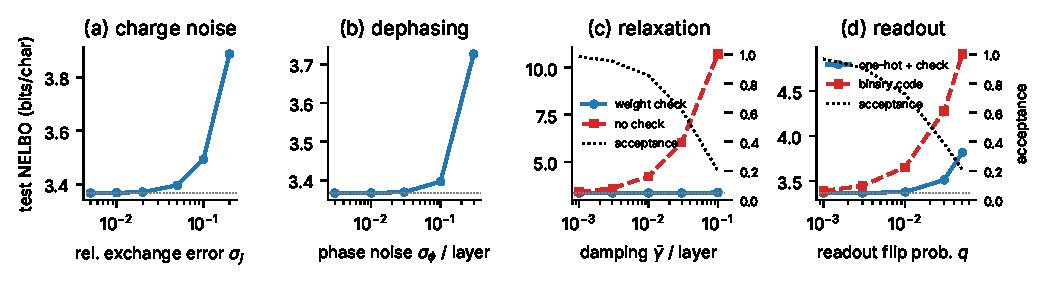
\includegraphics[width=0.92\textwidth]{figs/noise.pdf}
\caption{Test NELBO of the trained exchange denoiser (seed 0, 64 test windows, clean value 3.367 dotted)
under exactly simulated noise on all 32 qubits of every register.
(a) Quasi-static relative error of every exchange angle.
(b) Gaussian $Z$-phase per qubit per layer.
(c) Relaxation with qubit-dependent rates $\gamma_k\in[0.5,1.5]\bar\gamma$ per layer: Hamming-weight
check with post-selection (blue; dotted: acceptance) vs.\ no check, where a lost excitation is read as a
random token (red).
(d) Readout bit flips: one-hot register with weight check (blue; dotted: acceptance) vs.\ the same
distribution read out through a dense $\log_2V$-qubit binary code (red).}
\label{fig:noise}
\end{figure*}
Figure~\ref{fig:noise} shows the four noise channels of Sec.~\ref{sec:noise-theory}.
\emph{Charge noise}: a 2\% relative angle error costs $0.004$~bits/char and 5\% costs $0.03$.
\emph{Dephasing} up to $0.03$~rad per layer is negligible ($+0.003$).
\emph{Relaxation}: with the weight check the NELBO changes by less than $10^{-3}$~bits/char up to
$\bar\gamma=10^{-2}$ per layer, and rises by only $0.03$ at $\bar\gamma=0.1$, where 80\% of shots are
rejected. For uniform rates it is exactly unchanged ($3.3672$ at every $\gamma$), as predicted. Without the
check the same relaxation costs $0.07$ at $\bar\gamma=10^{-3}$ and $7.3$~bits/char at $0.1$.
\emph{Readout}: at $q=10^{-2}$ the one-hot register with weight check loses $0.012$ (acceptance 73\%),
while a binary code loses $0.29$. At $q=3\times10^{-2}$ the losses are $0.15$ and $0.91$.

\section{Discussion}
\paragraph{What the exchange read-out costs.} With identical features and controllers, replacing the
softmax by an exchange circuit plus a Born-rule measurement costs about $0.25$~bits/char
(linear controller: $3.38$ vs.\ $3.13$; MLP controller: $3.18$ vs.\ $2.92$). This happens even though
the circuit has more parameters, and Proposition~\ref{prop:reach} guarantees that every output
distribution is reachable. The gap is therefore one of \emph{parameterisation and optimisation}, not of
reachability. A softmax combines feature contributions additively in log space, i.e.\ as a product of
experts. Additive pulse areas instead interfere through a deep, periodic, non-commuting map, and the
sum rule of Prop.~\ref{prop:dark} couples all output amplitudes. The per-step decomposition
(Fig.~\ref{fig:per_t}) shows where the loss is incurred. Depth helps but saturates
(Table~\ref{tab:ablation}). Data re-uploading, which composes feature blocks non-commutatively, matched but did not beat additive
angles with the same block size, at much larger depth. The exchange envelope $J(t)$, which lets the device
turn its pulses off at low noise, gives a small but consistent gain ($0.024$~bits/char).

\paragraph{What the exchange read-out buys.} The read-out is native. Sampling requires one shot per token
per step, and the one-hot register makes the dominant hardware errors \emph{detectable}.
Relaxation, the most damaging channel without a check, becomes almost harmless with post-selection. It
is exactly harmless when rates are uniform. A single readout flip can never silently change a token.
For realistic readout errors ($q\approx10^{-2}$) the one-hot register loses $0.01$~bits/char, compared
with $0.29$ for a dense binary code (Fig.~\ref{fig:noise}). The model is also insensitive to
percent-level exchange miscalibration and to dephasing below $0.1$~rad per layer. These are regimes
reported for current silicon devices \citep{burkard2023semiconductor}.

\paragraph{Hardware cost.} One token per denoising step needs $V=32$ spins and, in the default
butterfly, 15 exchange layers (240 pulses). On a linear dot array the light cone forces at least $V-1$
brick-wall layers, and the 48-layer chain (744 pulses) matches the 240-pulse butterfly in quality. Positions
are conditionally independent within a step, so $L$ registers run in parallel and generation takes $T$
rounds of measure-and-reset. Butterfly connectivity needs long-range exchange (e.g.\ via shuttling).

\paragraph{Limitations.}
(i) \emph{Classical simulability.} A single excitation evolves like a single particle, so every result
here can be reproduced classically in $O(VG)$ time; this is how we trained. We make no claim of quantum
advantage. A natural extension that leaves the classically simulable regime is to let $k>1$ tokens
share one register. The Hamming-weight-$k$ sector has dimension $\binom{V}{k}$ and is still preserved by
exchange.
(ii) \emph{Local context.} All denoisers here see a fixed window of $\pm4$ noisy characters plus pair
features. Absolute numbers are therefore far from autoregressive models with longer context: an
interpolated Kneser--Ney 5-gram reaches $2.11$~bits/char on the same split \citep{chen1999empirical}.
We also trained a bidirectional Transformer denoiser with global context. Within our CPU budget it
stalled at the ``copy $x_t$ + unigram'' solution (test NELBO $4.23$~bits/char). We report it only in
the released logs, because it is not a well-tuned reference.
(iii) \emph{Small scale.} One corpus (\texttt{fortunes}, $2\times10^6$ characters), $V=32$ and $T=32$
steps. Uniform-transition diffusion is known to trail absorbing-state (masked) diffusion for text
\citep{austin2021structured,sahoo2024simple}. An exchange-only analogue of the absorbing state, for
example a dedicated ``mask'' qubit, is a natural next step.
(iv) \emph{Noise models.} Noise was injected at inference time into a model trained noise-free. We did
not model crosstalk, leakage out of the qubit manifold, or state-preparation errors.

\section{Conclusion}
A discrete diffusion language model can be built from the exchange interaction alone. Tokens are single
spin excitations, corruption is spin shuffling, and denoising is a context-controlled exchange circuit
read out by the Born rule. The exchange group on the token register is $\mathrm{U}(1)\oplus\mathrm{U}(V-1)$,
fixed by spin symmetry. It is small enough to avoid barren plateaus, yet large enough to reach every
categorical distribution. At equal features the exchange read-out trails a softmax by about $0.25$
bits/char. In return it comes with native one-shot sampling and built-in detection of relaxation and
readout errors. We hope these exact, reproducible baselines help calibrate claims about quantum
generative models of language.


\bibliographystyle{unsrtnat}
\bibliography{refs}
\end{document}
